\documentclass{article}

%% PAQUETES

% Paquetes generales
\usepackage[margin=2cm, paperwidth=210mm, paperheight=297mm]{geometry}
\usepackage[spanish]{babel}
\usepackage[utf8]{inputenc}
\usepackage{gensymb}

% Paquetes para estilos
\usepackage{textcomp}
\usepackage{setspace}
\usepackage{colortbl}
\usepackage{color}
\usepackage{color}
\usepackage{upquote}
\usepackage{xcolor}
\usepackage{listings}
\usepackage{caption}
\usepackage[T1]{fontenc}
\usepackage[scaled]{beramono}

% Paquetes extras
\usepackage{amssymb}
\usepackage{float}
\usepackage{graphicx}
\usepackage{url}

%% Fin PAQUETES


% Definición de preferencias para la impresión de código fuente.
%% Colores
\definecolor{gray99}{gray}{.99}
\definecolor{gray95}{gray}{.95}
\definecolor{gray75}{gray}{.75}
\definecolor{gray50}{gray}{.50}
\definecolor{keywords_blue}{rgb}{0.13,0.13,1}
\definecolor{comments_green}{rgb}{0,0.5,0}
\definecolor{strings_red}{rgb}{0.9,0,0}

%% Caja de código
\DeclareCaptionFont{white}{\color{white}}
\DeclareCaptionFont{style_labelfont}{\color{black}\textbf}
\DeclareCaptionFont{style_textfont}{\it\color{black}}
\DeclareCaptionFormat{listing}{\colorbox{gray95}{\parbox{16.78cm}{#1#2#3}}}
\captionsetup[lstlisting]{format=listing,labelfont=style_labelfont,textfont=style_textfont}

\lstset{
	aboveskip = {1.5\baselineskip},
	backgroundcolor = \color{gray99},
	basicstyle = \ttfamily\footnotesize,
	breakatwhitespace = true,   
	breaklines = true,
	captionpos = t,
	columns = fixed,
	commentstyle = \color{comments_green},
	escapeinside = {\%*}{*)}, 
	extendedchars = true,
	frame = lines,
	keywordstyle = \color{keywords_blue}\bfseries,
	language = Oz,                       
	numbers = left,
	numbersep = 5pt,
	numberstyle = \tiny\ttfamily\color{gray50},
	prebreak = \raisebox{0ex}[0ex][0ex]{\ensuremath{\hookleftarrow}},
	rulecolor = \color{gray75},
	showspaces = false,
	showstringspaces = false, 
	showtabs = false,
	stepnumber = 1,
	stringstyle = \color{strings_red},                                    
	tabsize = 2,
	title = \null, % Default value: title=\lstname
	upquote = true,                  
}

%% FIGURAS
\captionsetup[figure]{labelfont=bf,textfont=it}
%% TABLAS
\captionsetup[table]{labelfont=bf,textfont=it}

% COMANDOS

%% Titulo de las cajas de código
\renewcommand{\lstlistingname}{Código}
%% Titulo de las figuras
\renewcommand{\figurename}{Figura}
%% Titulo de las tablas
\renewcommand{\tablename}{Tabla}
%% Referencia a los códigos
\newcommand{\refcode}[1]{\textit{Código \ref{#1}}}
%% Referencia a las imagenes
\newcommand{\refimage}[1]{\textit{Imagen \ref{#1}}}


\begin{document}

% Inserción del título, autores y fecha.
\title{\Large 75.42 Taller de Programación I \\ 
	  \medskip\Huge Informe: Ejercicio N° 4  \\
	  \bigskip\Large\textit{``El código Draka (desencripción por fuerza bruta)''}}
\date{}
\maketitle




% INTRODUCCIÓN
\section{Introducción}
	
	Nuestros agentes finalmente han recuperado el código utilizado por los \textit{Draka} para encriptar y desencriptar sus mensajes. Si bien el código es relativamente simple, hasta el momento no ha sido posible encontrarle vulnerabilidades. Solo se sabe que los textos encriptados son ASCII \cite{ASCII} (códigos de carácter menores a 128) y que las claves solo utilizan dígitos ASCII. Aparentemente, debido a esto, la única opción para recuperar el texto será realizar un ataque de \textit{fuerza bruta} \cite{FB}.
	\par
	Las claves utilizadas son de longitud suficiente como para hacer que un ataque por fuerza bruta con una sola máquina lleve una excesiva cantidad de tiempo. Por lo tanto, se optará por una solución distribuida siguiendo un esquema cliente-servidor: el servidor se encargará de fraccionar el trabajo y los clientes de resolver cada una de estas partes, enviando los resultados al servidor.
	\par
	Detalles mas precisos de la problemática y de las condiciones preestablecidas se pueden encontrar en el enunciado del ejercicio\footnote{Se ha evitado hacer un relevamiento de la totalidad de la información que nos fue conferida, de manera de poder mantener el foco del informe en la forma en que se ha encarado la solución del problema.}.
\bigskip




% CONSIDERACIONES DE DISEÑO
\section{Consideraciones de diseño}

	Para la correcta implementación de la solución fue necesario plantear y establecer cómo se debería comportar el sistema ante ciertas situaciones que no fueron especificadas en el enunciado del problema. A continuación se listan las contemplaciones instauradas:

\begin{itemize}
	\itemsep=3pt \topsep=0pt \partopsep=0pt \parskip=0pt \parsep=0pt

	\item Al producirse una solicitud de trabajo por parte de un cliente, si el servidor le indica a este último que no hay trabajo para asignarle, entonces el cliente cerrará la conexión que los vinculaba y dará por finalizada su ejecución;

	\item El servidor almacenará todas las posibles claves enviadas por los clientes, de manera de que, una vez se indique la detención del mismo, se pueda determinar si existe una ambig\"uedad o si es única la clave;

	\item En el envío y en la recepción de datos se considera como fin de mensaje al caractér ``\textit{$\backslash$n}'' establecido por el protocolo.

	\item El programa del lado servidor no finalizará su ejecución a menos que se ingrese ``\textit{q$\backslash$n}'' por la entrada estándar.
\end{itemize}
\medskip




% DISEÑO
\section{Diseño}

	Como se mencionó anteriormente, se optará por una solución distribuida siguiendo un esquema cliente-servidor. De esta manera, poseeremos dos implementaciones independientes una de la otra, pero que trabajarán en conjunto una vez establecida la conexión entre las mismas. Por lo tanto, vamos a tener un programa \textit{servidor} y otro programa \textit{cliente}.
	\par
	En los apartados que siguen pondremos la atención en aquellos aspectos de la implementación de ambos programas que pueden ser relevantes a causa de su complejidad o particularidad. En estos se describen los inconvenientes que presentan y la forma en que fueron resueltos.
\bigskip



% DISEÑO - Cliente
\subsection{Cliente}
	
	Sin duda alguna, este ente del esquema es el menos complejo ya que su tarea se reduce a establecer inicialmente una conexión con el servidor, para luego solicitarle una parte del trabajo a realizar.
	\par
	En el caso de que el servidor le indique que no hay trabajo disponible, el cliente simplemente finalizará su ejecución. En la situación opuesta, recibirá un mensaje encriptado (codificado por el servidor en hexadecimal para su envío a través del socket) y el rango de claves, siendo su tarea probar cada una de ellas por fuerza bruta, notificando a través del socket cuales son posibles claves.
	\par
	Finalizadas las pruebas terminará su ejecución automáticamente dando fin a la conexión con el servidor.
	\par
	Debe tenerse en cuenta que ante cualquier problema surgido en la conexión, ya sea por una interrupción en la misma o por la llegada de mensajes erróneos que no se ajustan al protocolo u orden esperado, el programa cliente también finalizará su ejecución.
	\par
	Profundizando medianamente, este ente es implementado por la clase \textit{Cliente}, la cual, por las razones expuestas al inicio del apartado, se consideró que no sea un hilo independiente del programa invocante.
	\bigskip



% DISEÑO - Cliente - Pruebas sobre el código Draka
\subsubsection{Pruebas sobre el \textit{Código Draka}}

	Desde un principio se ha establecido que el cliente es el encargado de probar el rango de claves, asignado por el servidor, en el código utilizado por los Draka para encriptar y desencriptar sus mensajes.
	\par
	Para lograr una solución más elegante y mas limpia, se tomó la decisión de encapsular dicho código en una clase de métodos estáticos, \textit{CodigoDraga}, la que a su vez proporciona un método que recibe una clave y que se encarga de realizar la prueba sobre el código Draka, devolviendo como resultado de esta acción un valor lógico, es decir, si retorna ``true'' significará que la clave pasó la prueba y efectivamente puede ser considerada una posible clave, o si devuelve ``false'' la clave probada deberá ser descartada.
	\bigskip\bigskip


% DISEÑO - Servidor
\subsection{Servidor}

	Para el funcionamiento del servidor se ha propuesto utilizar una lógica muy simple. Esta consiste en tener a la clase \textit{Servidor}, la cual es un hilo de ejecución independiente del hilo principal del main, esperando por solicitudes de conexión por parte de los clientes. Cuando se recibe una petición de conexión por parte de un cliente, el mismo servidor se encarga de crear un objeto de la clase \textit{ConexionCliente}. A este objeto se le pasa el file descriptor correspondiente al nuevo socket que mantendrá en contacto al cliente con este último objeto. Además, el objeto que representa a la conexión será almacenado en una lista de conexiones existentes, para permitir al servidor saber que conexiones debe cerrar cuando llegue el momento de concluir la ejecución.
	\par
	Como se puede notar, esta clase, considerada la principal del lado servidor, simplemente se limita a la escucha a través de un socket, el cual solo es utilizado con este único fin. Todas las demás tareas de comunicación son derivadas y delegadas a las demás entidades, de las que haremos mención en los siguientes apartados.
	\bigskip\smallskip



% DISEÑO - Servidor - Conexion con el cliente
\subsubsection{Conexión con el cliente}

	Anteriormente se adelantó que la clase \textit{Servidor}, ante una nueva petición de conexión por parte de un host, creaba un objeto del tipo \textit{ConexionCliente}. Esto significa que este objeto es de ahora en más el único responsable del enlace con el cliente que realizó la petición, es decir, es el único encargado de mantener la comunicación con su par del otro lado del socket. Entre estos se hará el envío de mensajes protocolares los cuales permitirán la asignación de tareas, notificación de posibles claves, etc. Para esto, el ente que administra la conexión se mantendrá en estrecha relación con el \textit{controlador de tareas} del servidor.
	\bigskip\smallskip



% DISEÑO - Servidor - Control de tareas
\subsubsection{Control de tareas}

	Otro de los entes que se encuentra a las ordenes del servidor, ya que es creado por este mismo y no puede existir mas allá del alcance de este, es el representado por la clase \textit{ControladorDeTareas}. Como su nombre lo indica, es el encargado de administrar las tareas. Más especificamente, su labor está centrada en:
	\medskip

	\begin{itemize}
		\itemsep=3pt \topsep=0pt \partopsep=0pt \parskip=5pt \parsep=0pt

		\item \textit{División de tareas}: deberá fraccionar las partes de trabajo que deben ser asignadas a cada cliente, como así también indicar cuando ya no hay mas tareas por repartir;

		\item \textit{Recepción de claves}: cada objeto del tipo \textit{ConexionCliente}, al recibir una clave de parte del cliente notificará al controlador de tareas despachándole esta misma clave;

		\item \textit{Finalización de tarea}: cuando un cliente envía el mensaje de que ha concluido con su parte del trabajo, el objeto \textit{ConexionCliente} asociado a dicha conexión notificará al controlador de tareas de tal evento;

		\item \textit{Notificar estado de tareas}: deberá informarle al servidor del estado de las tareas cuando este lo solicite.

	\end{itemize}
	\bigskip


	De estas cuatro labores debemos destacar una en particular: la \textit{recepción de claves}. Esto se debe a que presenta una de las problemáticas mas interesantes. 
	\par
	Tal como se mencionó, el controlador de tareas recibirá las claves, pero hay que tener en cuenta que cada objeto \textit{ConexionCliente} se encuentra corriendo en un hilo independiente y que se puede dar el caso de que dos de estos hilos traten de notificar al mismo tiempo la llegada de una nueva clave. Es aquí donde se decidió convertir a la clase \textit{ControladorDeTareas} en thread-safe, es decir, con soporte para multithreading. Por lo tanto, se incluyó una auto protección (un objeto de tipo \textit{Mutex}) en la clase, lo cual evita que las instancias de esta misma sean accedidas al mismo tiempo por hilos diferentes.
	\par
	Por otro lado, al ser informado de la llegada de una nueva clave, el controlador de tareas debe tomar a esta última e ingresarla en una lista proporcionada por la clase \textit{Servidor}. Esta lista presenta problemas semejantes con respecto al multithreading, razón por la cual será discutida en el apartado que sigue, dándose detalles de cómo es que se evitan los conflictos de acceso a un objeto por parte de múltiples hilos.
	\bigskip\smallskip



% DISEÑO - Servidor - Clase Lista
\subsubsection{Clase \textit{Lista}}
	
	Como ya es sabido, la \textit{STL} \cite{STL} no proporciona estructuras con soporte para multithreading. Este es el caso del contenedor \textit{list}, el cual no es \textit{thread-safe}. Ante la necesidad de la utilización de esta en el lado del servidor, de manera de poder albergar a las claves que arriven desde los clientes (como se explicó en el apartado anterior), es que se decidió extender a \textit{list} y agregarle el debido soporte.
	\par
	Para esto, hemos creado una clase \textit{Lista}, la cual utiliza internamente al contenedor \textit{list}, pero con la salvedad de que cada método se encuentra protegido de los múltiples accesos posibles desde distintos threads. 
	\par
	Es así que se estableció como un atributo interno y privado un objeto de tipo \textit{Mutex}, el cual es bloqueado en cada invocación a los métodos, evitando que mientras se ejecutan las instrucciónes de este último, otros threads puedan hacer uso de la lista, quedando en su defecto a la espera de la liberación del mutex.
	\bigskip\medskip




% PROTOCOLO Y COMUNICACION
\subsection{Protocolo y comunicación}

	Respecto a la forma en que se comunican los clientes y el servidor, ya se adelantó anteriormente la utilización de un protocolo fijo e irremplazable. Para poder unificarlo y que los objetos comprendan los mismos tipos de mensajes se creó la clase \textit{Protocolo}, la cual simplemente alberga constantes que definen los distintos tipos de avisos a intercambiar entre los entes.
	\par
	Por otro lado, para abstraer la forma de enviar y recibir datos, se decidió establecer como intermediario a la clase \textit{Comunicador}, la cual se encarga de emitir o de recibir datos (a través del socket proporcionado por su empleador) teniendo en cuenta el protocolo antes mencionado.
	\bigskip\bigskip




% FUTURAS MEJORAS
\section{Futuras mejoras}

	Se listan aquí posibles mejoras a realizar en el futuro, como así también, ciertas falencias que fueron descubiertas habiéndose hecho ya la entrega del producto, a fin de denotar conciencia sobre el trabajo realizado:

	\begin{itemize}
		\itemsep=3pt \topsep=0pt \partopsep=0pt \parskip=0pt \parsep=0pt

		\item Mejorar informe de errores en clase \textit{Cliente}, de manera de proporcionar información mas detallada acerca de la desconexión del socket;

		\item Clases \textit{Thread} y \textit{Mutex} mas completas con respecto al soporte de mas opciones;

		\item Mejorar empaquetamiento de la clase \textit{Comunicador} y el armado de mensajes por parte de este.

	\end{itemize}
	\bigskip
\newpage




% ESQUEMA DEL DISEÑO
\section{Esquema del diseño}

	A continuación, en la \textit{Figura 1}, se ilustra el diagrama de clases principal, donde se pueden ver las entidades que intervienen tanto en el
	servidor como así también en el cliente. Cabe destacar que se han omitido,
	para mayor comprensión, ciertas clases secundarias que hacen a la totalidad del sistema, pero que su presencia no es indispensables para el entendimiento del funcionamiento general del mismo. 
	\bigskip\bigskip\bigskip\bigskip


% Figura 1
\begin{figure}[h]
	\centering
	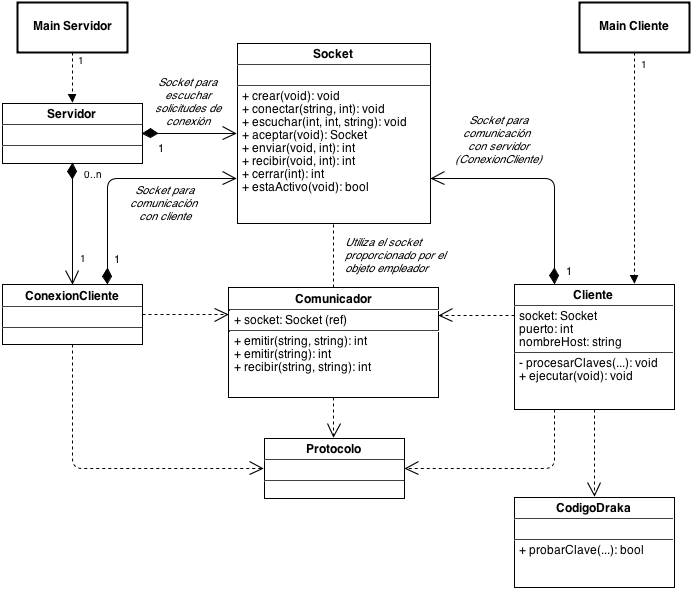
\includegraphics[width=0.9465\textwidth]{images/diagrama_p1.png}
	\medskip
	\caption{Diagrama de clases principal del cliente-servidor.}
\end{figure}
\bigskip\bigskip\bigskip\bigskip

	
	Por último, en la \textit{Figura 2}, se muestra un diagrama de clases ampliado del lado servidor. En este se ilustra qué clases son un \textit{Thread}, es decir, que clases proveen objetos que corren en distintos hilos al ser instanciadas. Además se puede observar la relación entre entidades, las cuales fueron descriptas en secciones anteriores.

\newpage
% Figura 2
\begin{figure}[h]
	\centering
	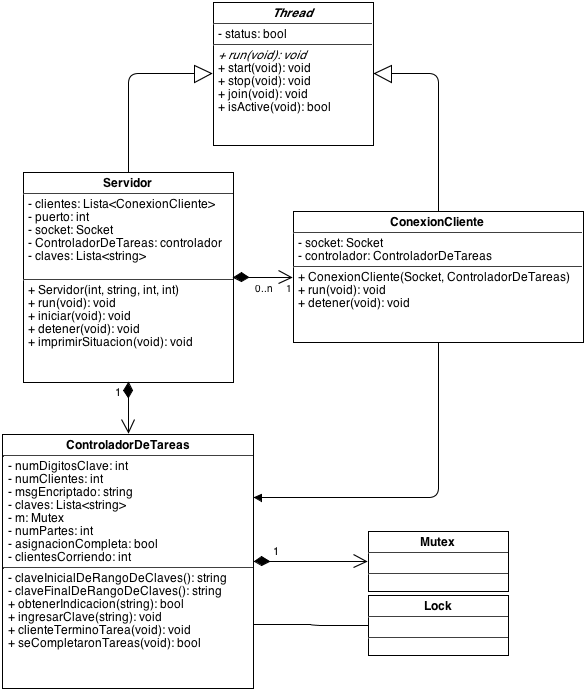
\includegraphics[width=0.8\textwidth]{images/diagrama_p2.png}
	\medskip
	\caption{Diagrama de clases del servidor.}
\end{figure}
\bigskip\bigskip\bigskip\bigskip




% REFERENCIAS
\begin{thebibliography}{99}

	\bibitem{ASCII} Código ASCII, \url{http://en.wikipedia.org/wiki/ASCII}
	\bibitem{FB} Ataque por Fuerza Bruta (Brute-force attack), \url{http://en.wikipedia.orig/wiki/Brute-force_attack}
	\bibitem{STL} Standard Template Library, \url{http://en.wikipedia.org/wiki/Standard_Template_Library}
	\end{thebibliography}






\end{document}
